\documentclass[aspectratio=169,10pt]{beamer}

\usepackage{amsmath,amssymb,bm,booktabs,graphicx,microtype}
\usepackage{array}

\definecolor{navy}{HTML}{17324D}
\definecolor{blue}{HTML}{2C6E9B}
\definecolor{gold}{HTML}{E69F00}
\definecolor{green}{HTML}{009E73}
\definecolor{purple}{HTML}{332288}
\definecolor{orange}{HTML}{D55E00}
\definecolor{softgray}{HTML}{F2F5F7}
\definecolor{midgray}{HTML}{5F6B73}

\setbeamercolor{normal text}{fg=navy,bg=white}
\setbeamercolor{structure}{fg=blue}
\setbeamercolor{frametitle}{fg=white,bg=navy}
\setbeamercolor{title}{fg=white}
\setbeamercolor{subtitle}{fg=white}
\setbeamercolor{author}{fg=white}
\setbeamercolor{date}{fg=white}
\setbeamercolor{block title}{fg=white,bg=blue}
\setbeamercolor{block body}{fg=navy,bg=softgray}
\setbeamercolor{alerted text}{fg=orange}
\setbeamerfont{frametitle}{series=\bfseries,size=\large}
\setbeamerfont{title}{series=\bfseries,size=\LARGE}
\setbeamerfont{subtitle}{size=\large}
\setbeamerfont{footline}{size=\scriptsize}
\setbeamertemplate{navigation symbols}{}
\setbeamertemplate{itemize item}{\color{gold}$\blacktriangleright$}
\setbeamertemplate{itemize subitem}{\color{blue}$\bullet$}
\setbeamertemplate{frametitle}{%
  \nointerlineskip
  \begin{beamercolorbox}[wd=\paperwidth,ht=0.75cm,dp=0.22cm,leftskip=0.45cm]{frametitle}
    \insertframetitle
  \end{beamercolorbox}}
\setbeamertemplate{footline}{%
  \leavevmode%
  \hbox{%
    \begin{beamercolorbox}[wd=.82\paperwidth,ht=2.6ex,dp=1.1ex,leftskip=.45cm]{author in head/foot}%
      \color{midgray}Softmax-kernel in-context Bayesian near-field LSM
    \end{beamercolorbox}%
    \begin{beamercolorbox}[wd=.18\paperwidth,ht=2.6ex,dp=1.1ex,rightskip=.45cm plus1fil]{date in head/foot}%
      \color{midgray}\hfill\insertframenumber/\inserttotalframenumber
    \end{beamercolorbox}}}

\newcommand{\metric}[2]{%
  \begin{beamercolorbox}[rounded=true,sep=0.55em,wd=\linewidth]{block body}
    {\color{gold}\bfseries #1}\hfill {\bfseries #2}
  \end{beamercolorbox}}
\newcommand{\smallsource}{\par\vspace{0.10em}{\tiny\color{midgray}Held-out simulated near-field tasks; CG claims use the common physical residual.}}

\title{What Did Context-PCG Learn?}
\subtitle{Softmax-kernel in-context Bayesian near-field linear sampling}
\author{Janis and Hancya}
\date{August 2026}

\begin{document}

{
\setbeamertemplate{footline}{}
\setbeamercolor{background canvas}{bg=navy}
\begin{frame}[plain]
  \vfill
  \titlepage
  \vfill
  \begin{center}
    \color{gold}\rule{0.60\textwidth}{1.3pt}
  \end{center}
\end{frame}
}

\begin{frame}{The question: can the prompt teach us how to condition?}
\begin{columns}[T,onlytextwidth]
\begin{column}{0.55\textwidth}
  \begin{block}{Bayesian near-field LSM requires two coupled solves}
  \begin{equation*}
    H_DQ_\mu=\Phi,\qquad H_DQ_\Sigma=N_DK_\Gamma .
  \end{equation*}
  \begin{equation*}
    M_D=K_\Gamma N_D^*Q_\mu,\qquad
    \Sigma_D=K_\Gamma-K_\Gamma N_D^*Q_\Sigma .
  \end{equation*}
  \end{block}
  \begin{itemize}
    \item Original two-dimensional near-field acquisition.
    \item Deterministic point sources and receivers; one to six sound-soft obstacles.
    \item Mean accuracy alone is insufficient: the covariance solve controls numerical UQ.
  \end{itemize}
\end{column}
\begin{column}{0.41\textwidth}
  \metric{Severe ill-conditioning}{$\kappa(H_D)$ up to $2.7\times10^4$}
  \vspace{0.55em}
  \metric{Matched budget}{$T=32$ operator applications}
  \vspace{0.55em}
  \metric{Core comparison}{context-PCG vs CG}
  \vspace{0.8em}
  \begin{alertblock}{Modelling choice}
  The softmax/von-Mises nonlinearity fixes the GP feature space; it is not a learned temperature.
  \end{alertblock}
\end{column}
\end{columns}
\end{frame}

\begin{frame}{The learned object: one SPD factor per prompt}
\begin{columns}[T,onlytextwidth]
\begin{column}{0.57\textwidth}
  \begin{equation*}
  C_\theta(D,\Gamma)=U_\Gamma
  \operatorname{diag}\!\left[g_\theta(U_\Gamma^*H_DU_\Gamma)\right]^{1/2}
  U_\Gamma^*,\qquad g_\theta>0 .
  \end{equation*}
  \begin{equation*}
    \widetilde H_D=C_\theta^*H_DC_\theta,\qquad q=C_\theta x .
  \end{equation*}
  \begin{itemize}
    \item The encoder reads the diagonal, row-$\ell_1$, and row-$\ell_2$ norms of the prompt Hessian in the fixed GP basis.
    \item Shared token maps and mean pooling allow variable context length.
    \item The factor is computed once and frozen for all iterations: this remains standard PCG, not flexible CG.
  \end{itemize}
\end{column}
\begin{column}{0.39\textwidth}
  \begin{block}{What is learned}
    Positive, task-dependent modal gains.
  \end{block}
  \begin{block}{What is not learned}
    The softmax kernel, an obstacle image, the LSM indicator, or a spatial regularization map.
  \end{block}
  \begin{alertblock}{Architectural restriction}
    Modal gains cannot rotate obstacle-dependent eigendirections outside $U_\Gamma$.
  \end{alertblock}
\end{column}
\end{columns}
\end{frame}

\begin{frame}{What was learned? Four controls isolate the signal}
\small
\renewcommand{\arraystretch}{1.25}
\setlength{\tabcolsep}{3pt}
\begin{tabular}{>{\raggedright\arraybackslash}p{0.20\textwidth} >{\raggedright\arraybackslash}p{0.25\textwidth} >{\centering\arraybackslash}p{0.14\textwidth} >{\raggedright\arraybackslash}p{0.31\textwidth}}
\toprule
Method & Information available & Physical gain over CG & Interpretation \\
\midrule
population-PCG & Acquisition distribution only & $1.58\times$ & Shared geometry helps, but fails under strong joint shift ($0.42\times$). \\
context-PCG & Current task Hessian statistics & $\mathbf{2.05\times}$ & The prompt contains useful task-specific conditioning signal. \\
angular-Jacobi PCG & Exact current diagonal in GP basis & $1.70\times$ & Most available signal is cheaply accessible analytically. \\
hybrid-PCG & Analytic base + bounded learned correction & $1.69\times$ & The residual network adds no robust signal in the fixed basis. \\
\bottomrule
\end{tabular}

\vspace{0.75em}
\begin{alertblock}{Main inference}
Context-PCG learns finite-horizon, task-dependent spectral weighting beyond a population factor. It does \emph{not} learn a universally superior preconditioner: a correctly specified analytic GP-basis factor remains the stronger wall-clock control.
\end{alertblock}
\smallsource
\end{frame}

\begin{frame}{Scaling study: what was actually run}
\small
\begin{columns}[T,onlytextwidth]
\begin{column}{0.31\textwidth}
  \metric{Dataset size}{$128\rightarrow32{,}768$}
  \vspace{0.35em}
  \metric{Network width}{$32\rightarrow512$}
  \vspace{0.35em}
  \metric{Context size}{$8\rightarrow48$}
  \vspace{0.35em}
  \metric{Depth}{$1\rightarrow128$}
\end{column}
\begin{column}{0.31\textwidth}
  \metric{Trained models}{90}
  \vspace{0.35em}
  \metric{Dataset checkpoints}{810}
  \vspace{0.35em}
  \metric{Task evaluations}{362,880}
  \vspace{0.35em}
  \metric{Frozen seeds}{3}
\end{column}
\begin{column}{0.33\textwidth}
  \scriptsize
  \begin{block}{Matched learned solvers}
  population-PCG, context-PCG, hybrid-PCG, Richardson, heavy-ball, Chebyshev.
  \end{block}
  \begin{block}{Training-free controls}
  CG, optimized CG, physical Jacobi, block-Jacobi, angular-Jacobi, exact dense solve.
  \end{block}
  \begin{block}{Audits}
  Independent geometries, obstacle count, noise, aperture, frequency, joint shift, time, and UQ.
  \end{block}
\end{column}
\end{columns}
\end{frame}

\begin{frame}{Direct answer versus ordinary CG}
\centering
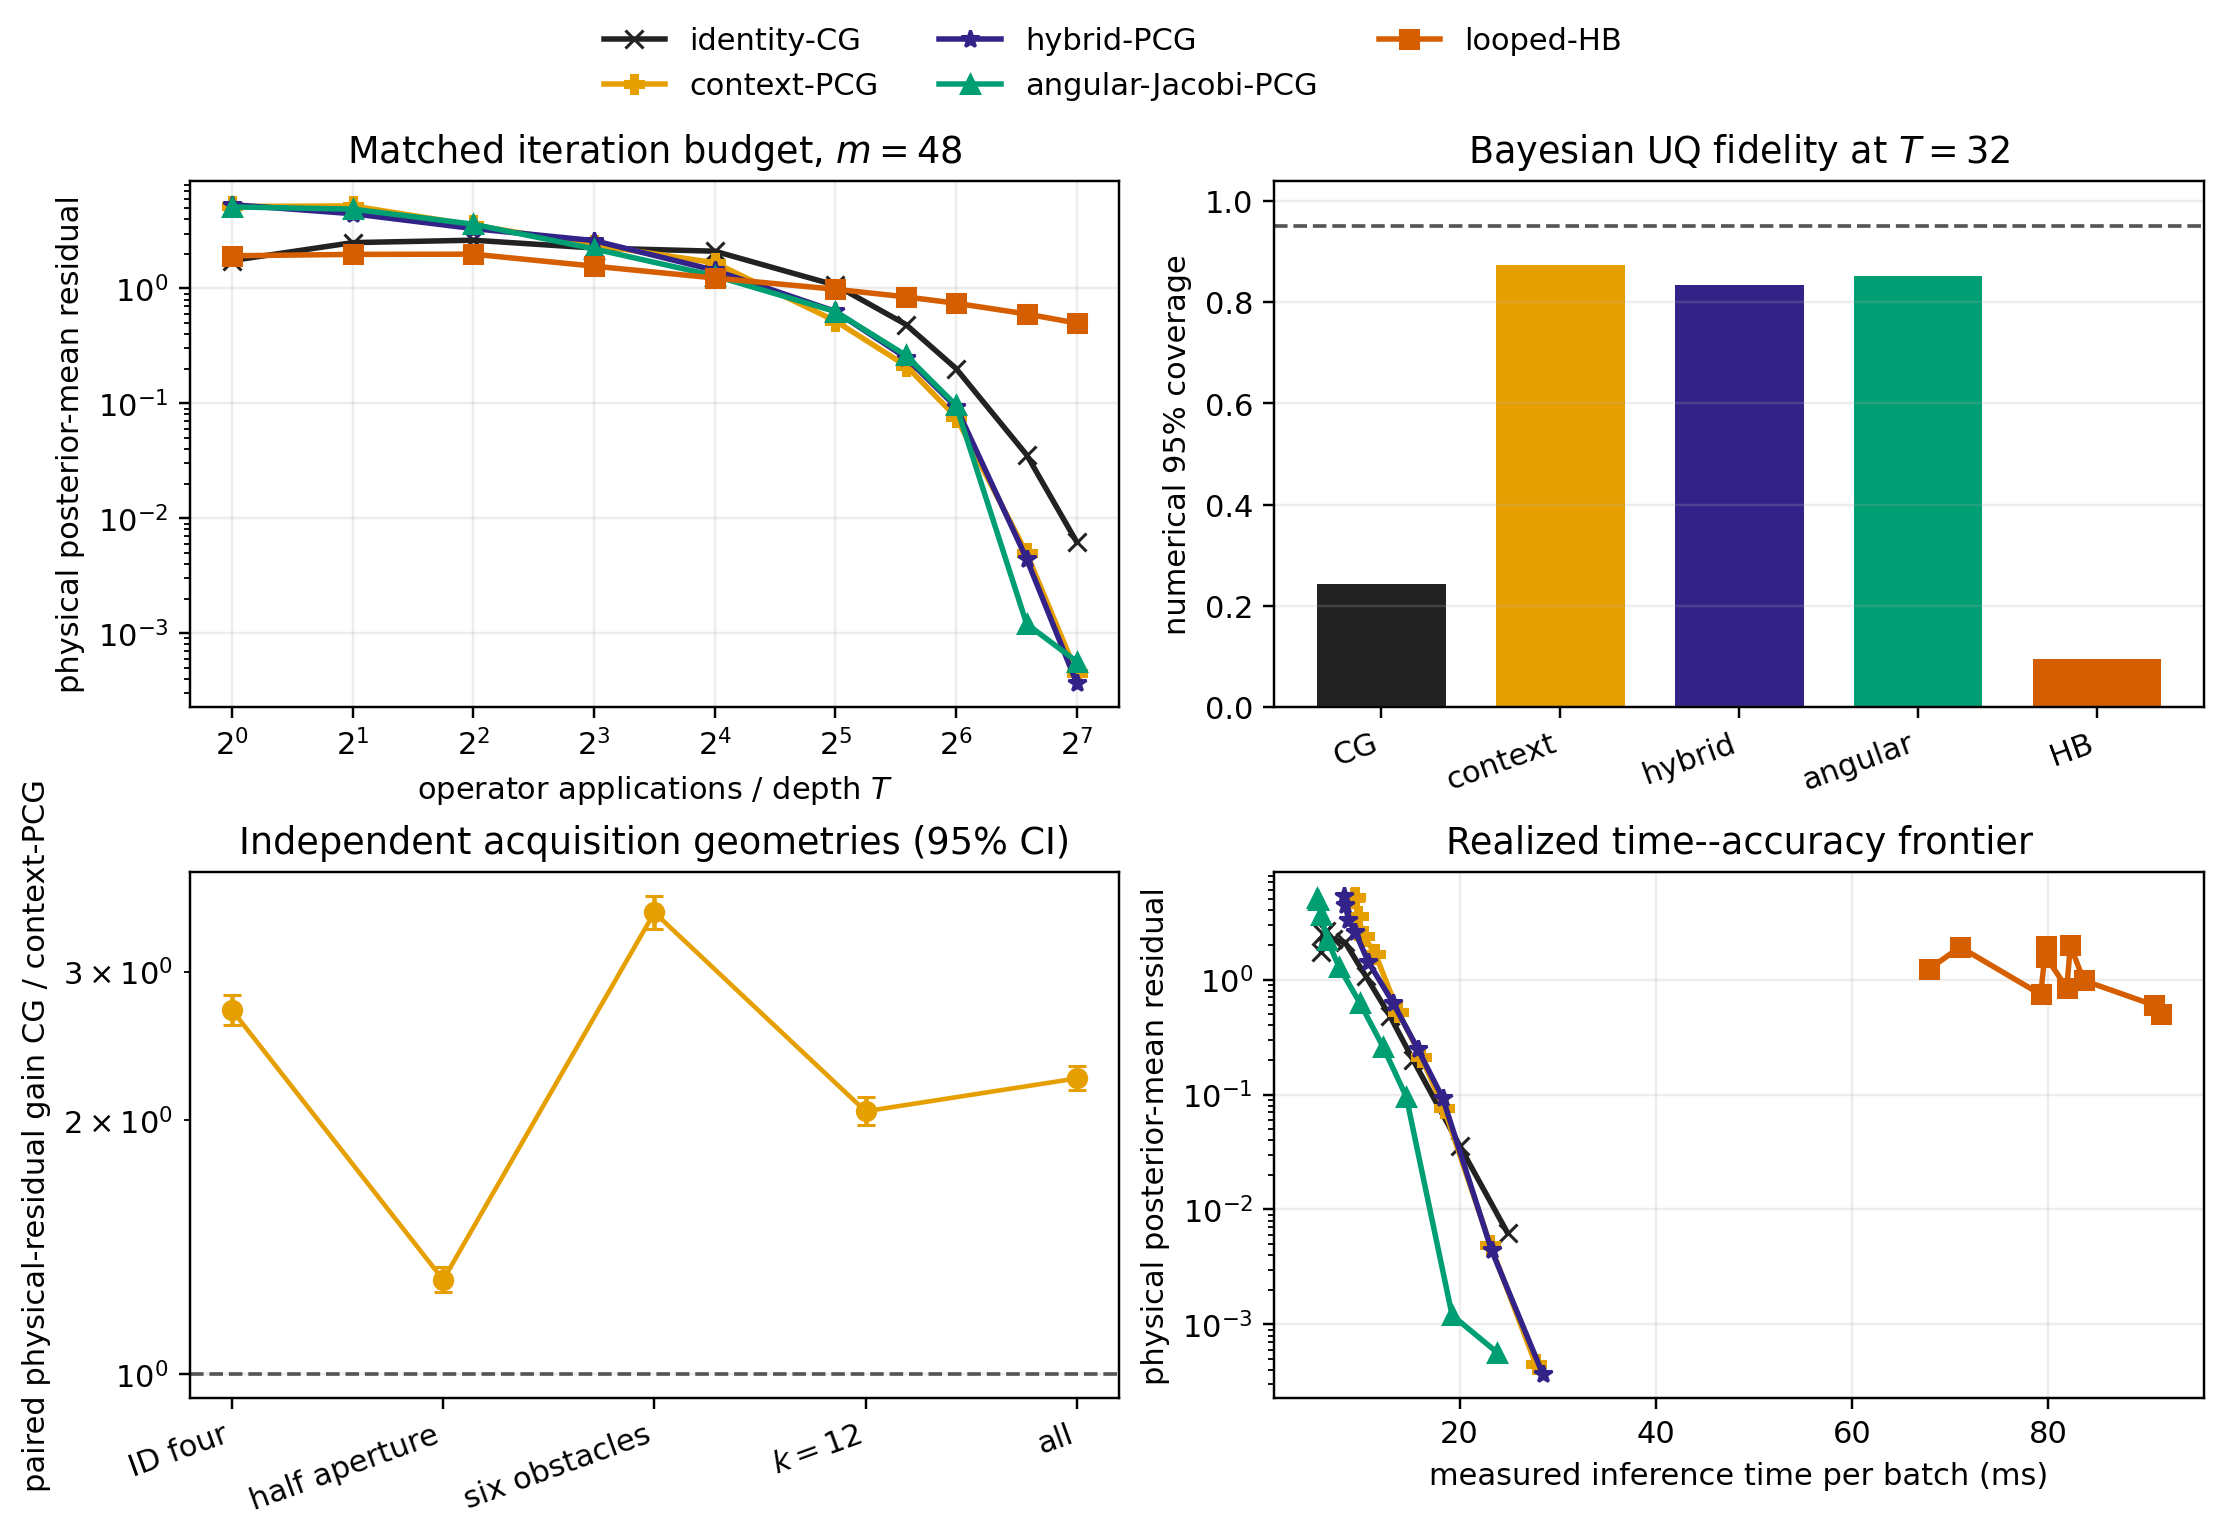
\includegraphics[width=0.86\textwidth,height=0.74\textheight,keepaspectratio]{scaling_cg_comparison.png}
\vspace{-0.25em}
\begin{columns}[onlytextwidth]
\begin{column}{0.32\textwidth}\centering
  {\color{gold}\bfseries $2.05\times$} physical-residual gain
\end{column}
\begin{column}{0.32\textwidth}\centering
  {\color{gold}\bfseries $6.44\times$} lower score error
\end{column}
\begin{column}{0.32\textwidth}\centering
  Coverage: {\bfseries $0.243\rightarrow0.873$}
\end{column}
\end{columns}
\par\vspace{0.15em}{\scriptsize\color{midgray}Learned stationary loops remain inferior: even heavy-ball gives only $1.09\times$, AP $0.478$, coverage $0.095$, and 83.6 ms.}
\end{frame}

\begin{frame}{Conditioning mechanism: useful compression, incomplete basis}
\begin{columns}[T,onlytextwidth]
\begin{column}{0.68\textwidth}
  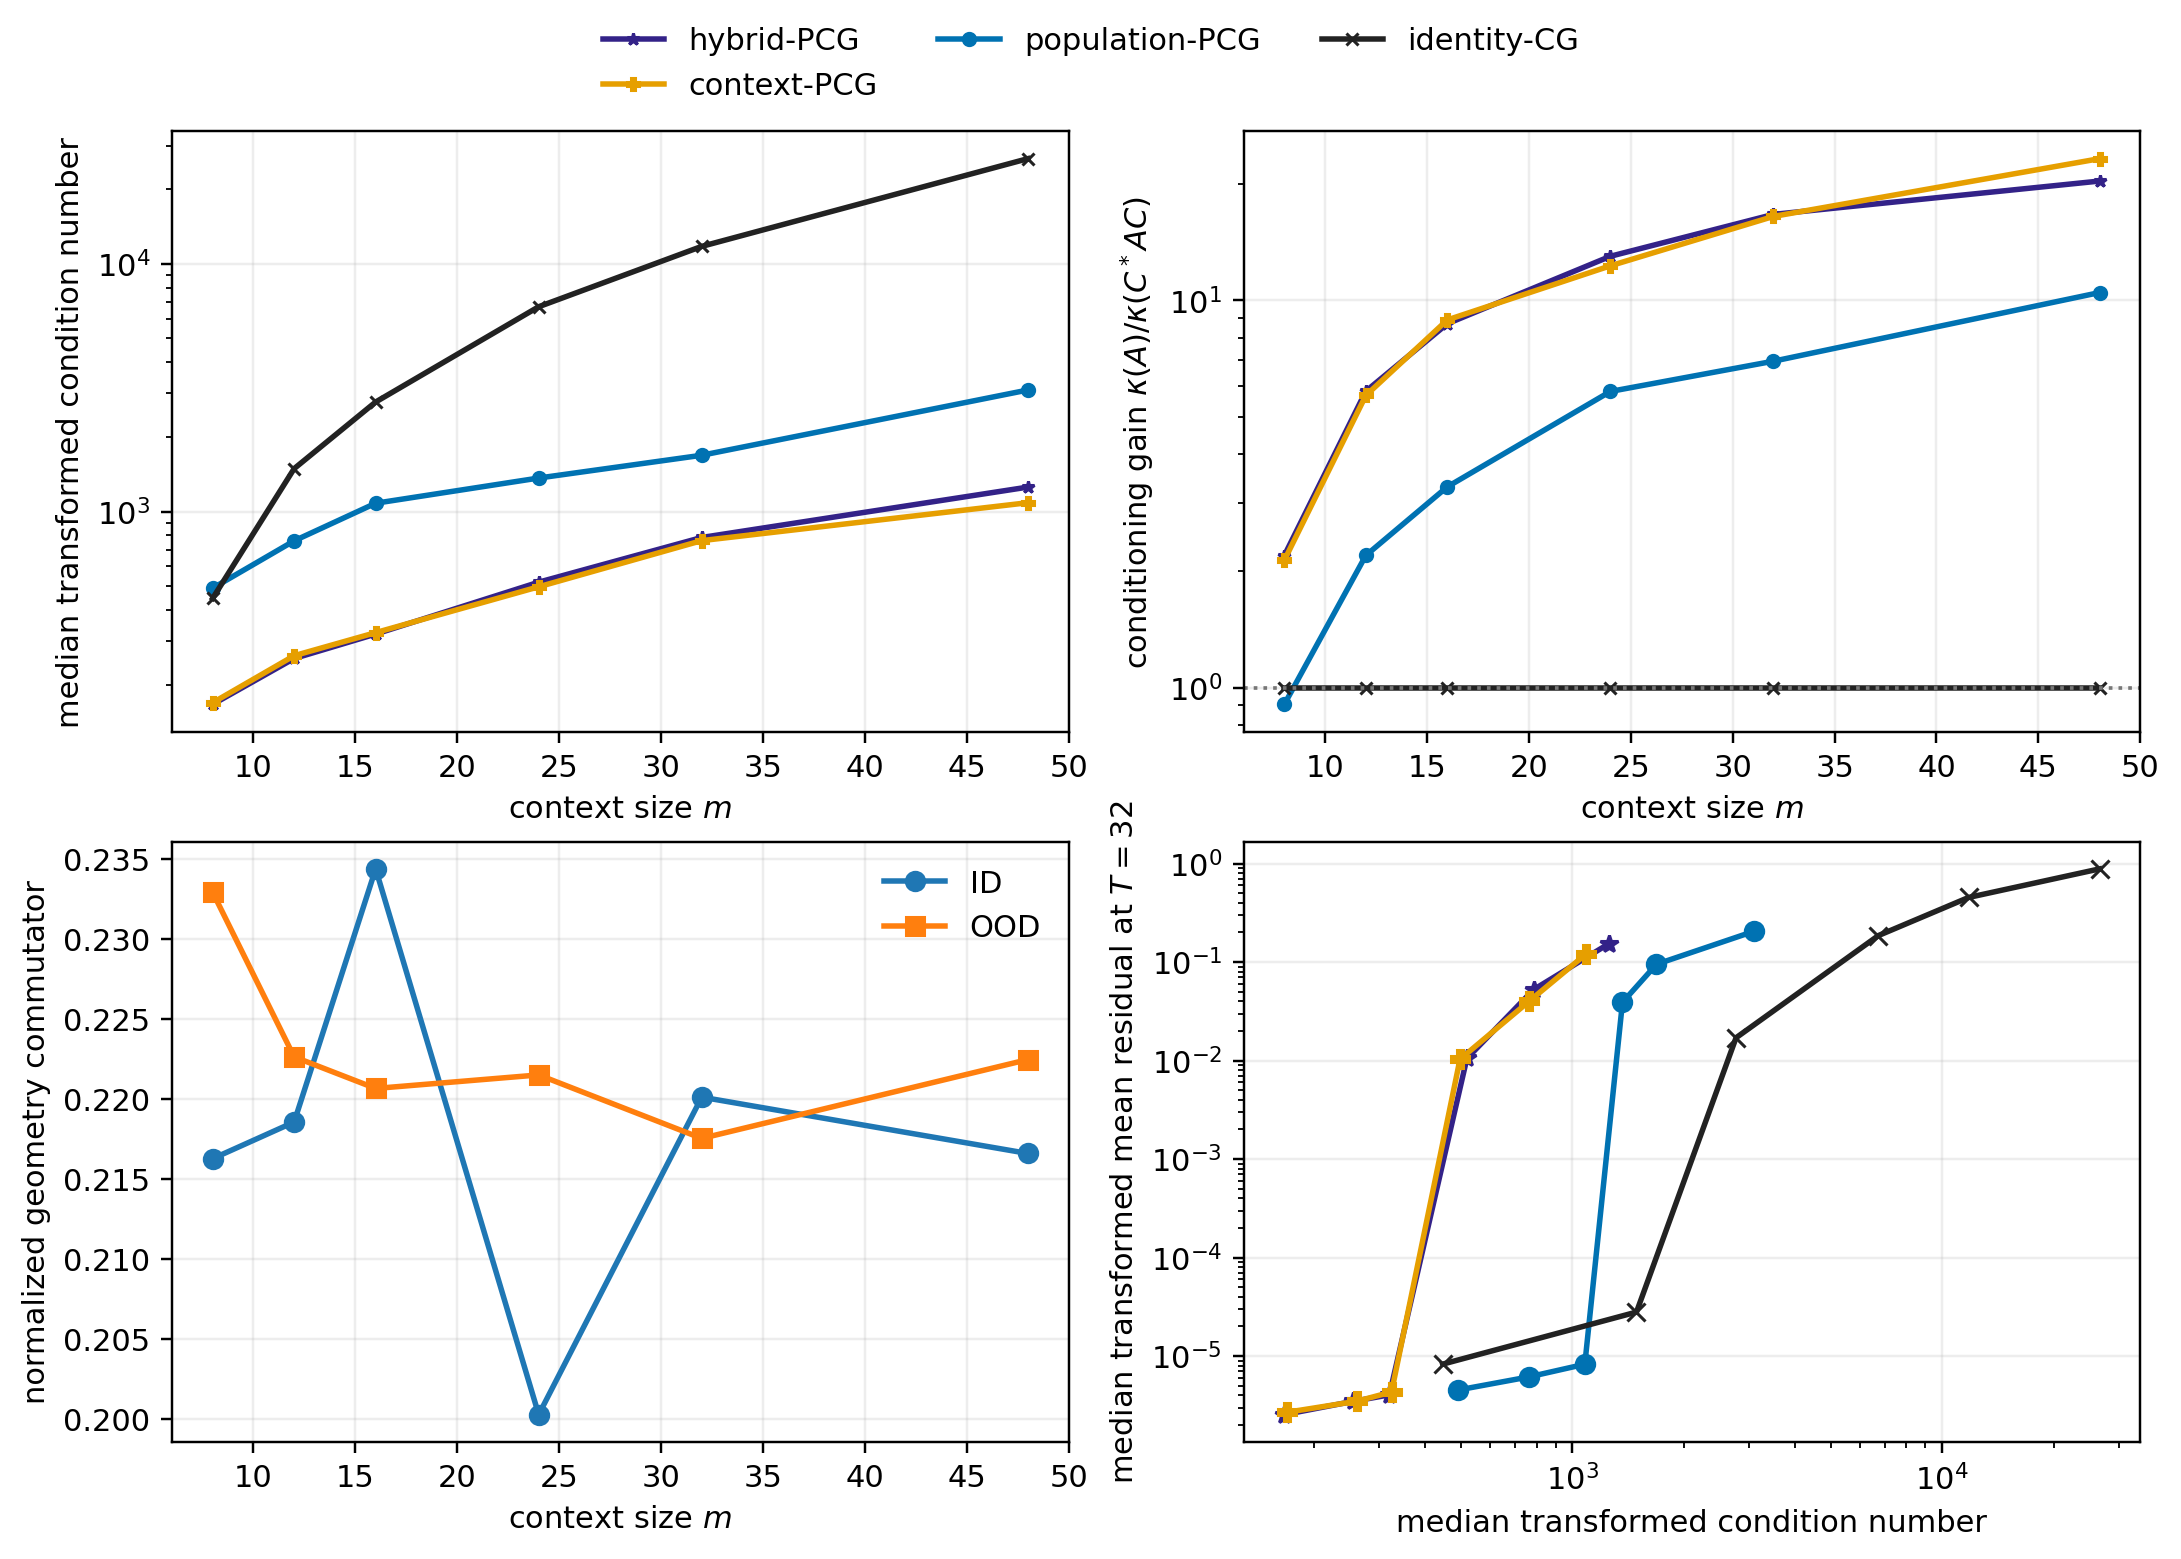
\includegraphics[width=\linewidth,height=0.70\textheight,keepaspectratio]{scaling_conditioning.png}
\end{column}
\begin{column}{0.29\textwidth}
  \small
  \metric{Raw median $\kappa$}{$2.66\times10^4$}
  \vspace{0.55em}
  \metric{Context-PCG}{$23.22\times$ reduction}
  \vspace{0.55em}
  \metric{Angular-Jacobi}{$24.28\times$ reduction}
  \vspace{0.45em}
  \begin{alertblock}{What $\kappa$ misses}
  Similar condition numbers can yield different finite-depth residuals: clustering and right-hand-side alignment also matter.
  \end{alertblock}
\end{column}
\end{columns}
\end{frame}

\begin{frame}{Robustness: prompt conditioning survives physical shifts}
\centering
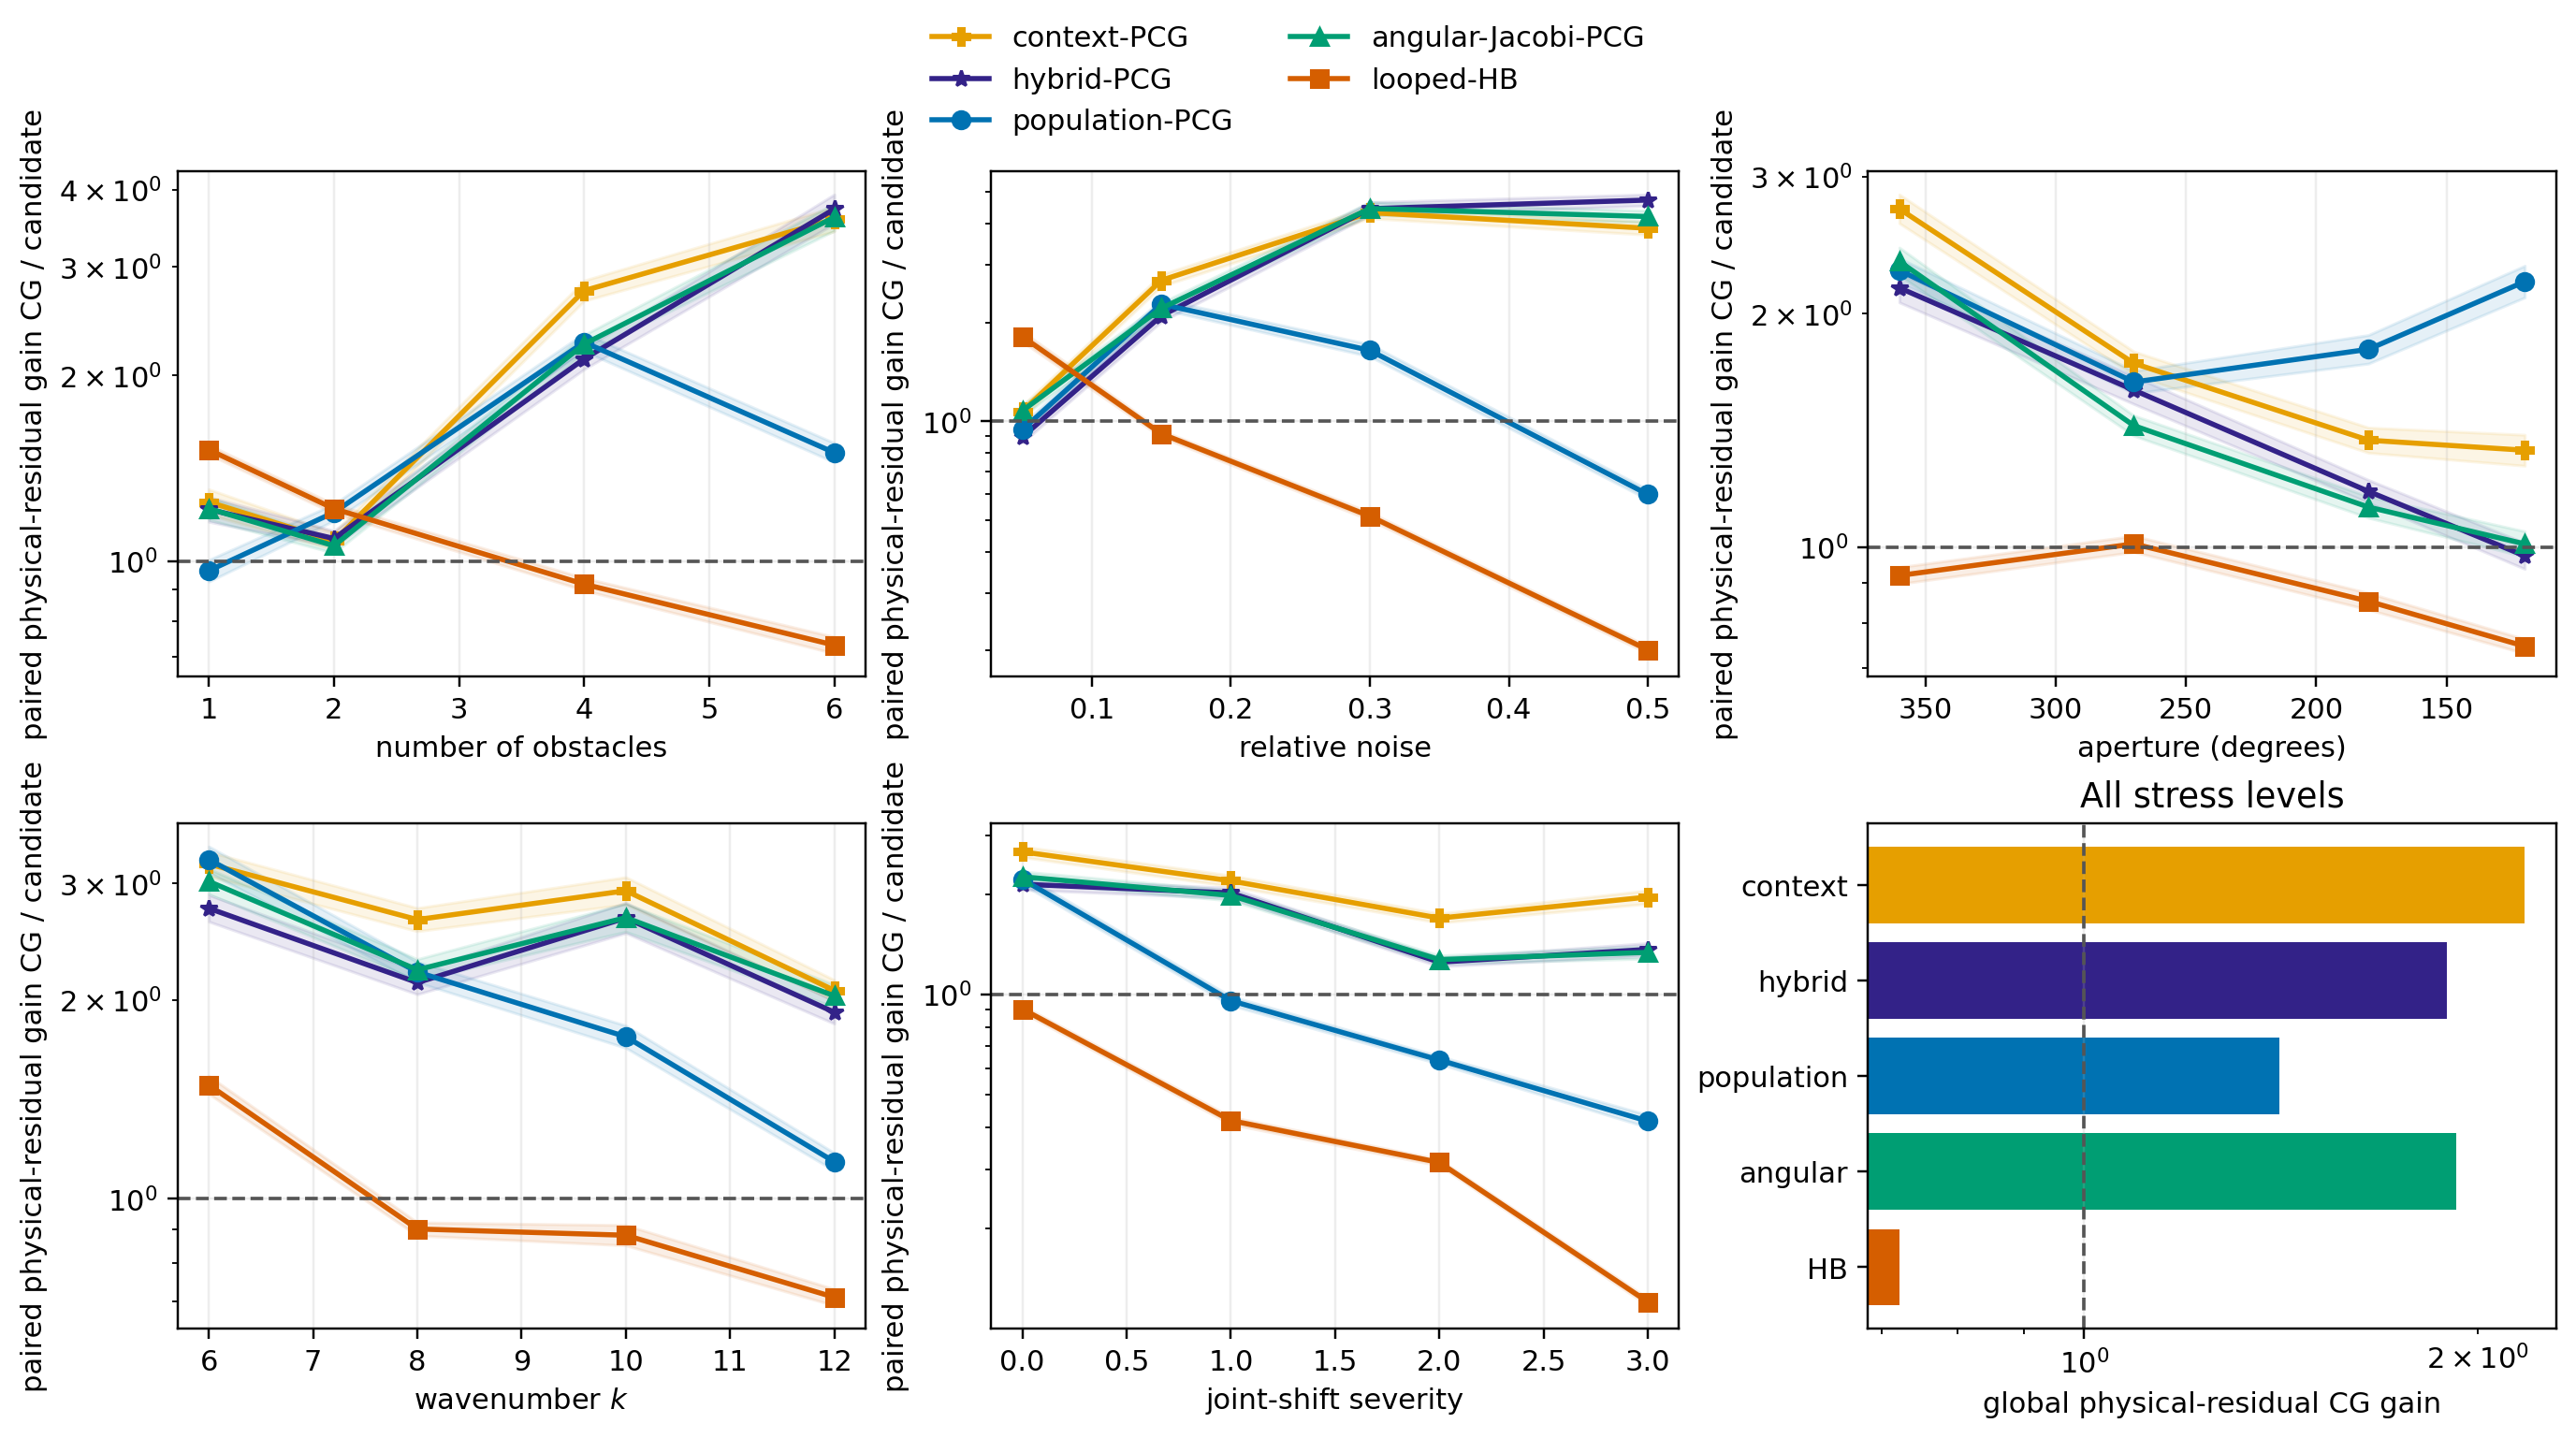
\includegraphics[width=0.86\textwidth,height=0.74\textheight,keepaspectratio]{scaling_cg_stress_test.png}
\vspace{-0.2em}
\begin{columns}[onlytextwidth]
\begin{column}{0.32\textwidth}\centering
  Gain range: {\bfseries $1.07\times$--$4.32\times$}
\end{column}
\begin{column}{0.32\textwidth}\centering
  All context-PCG 95\% lower bounds $>1$
\end{column}
\begin{column}{0.32\textwidth}\centering
  Extreme joint shift: {\bfseries $1.96\times$}
\end{column}
\end{columns}
\smallsource
\end{frame}

\begin{frame}{Learned versus informed analytic PCG}
\begin{columns}[T,onlytextwidth]
\begin{column}{0.64\textwidth}
  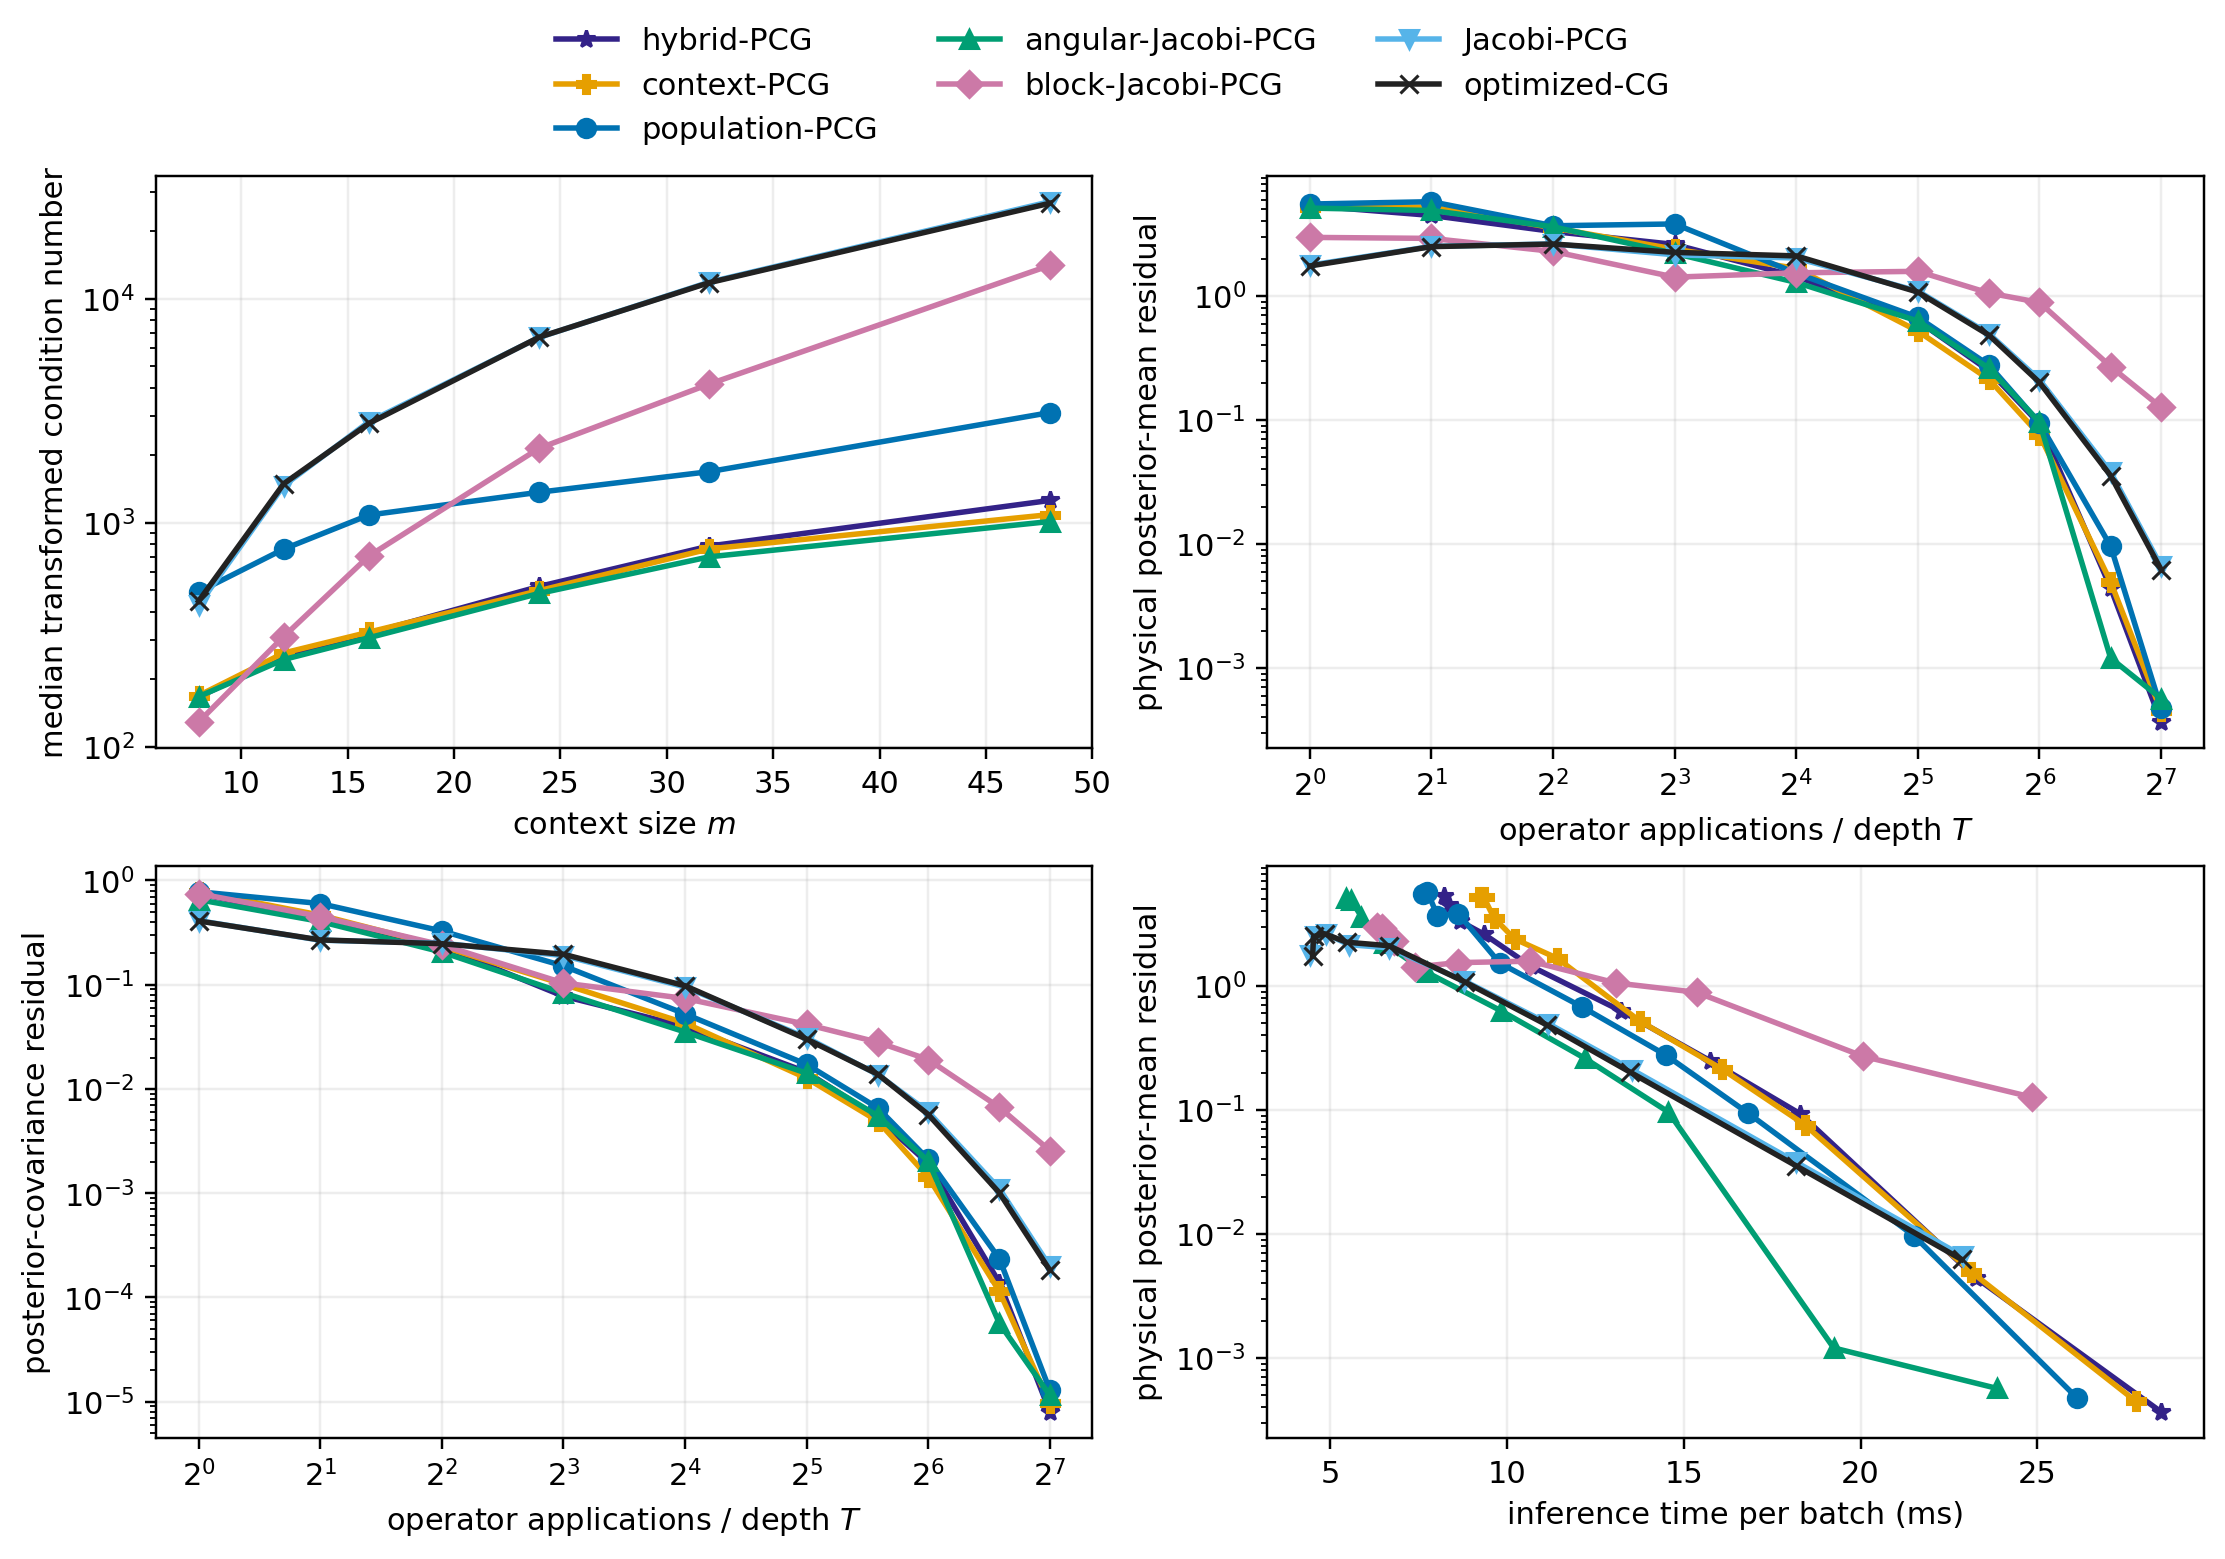
\includegraphics[width=\linewidth,height=0.68\textheight,keepaspectratio]{scaling_classical_preconditioners.png}
\end{column}
\begin{column}{0.33\textwidth}
  \small
  \begin{block}{At $m=48$, $T=32$}
  \begin{itemize}\setlength\itemsep{0.1em}
    \item context-PCG residual: \textbf{0.521}
    \item angular-Jacobi residual: \textbf{0.629}
    \item angular-Jacobi is faster: \textbf{9.84 ms} vs \textbf{13.75 ms}
  \end{itemize}
  \end{block}
  \begin{alertblock}{Correct interpretation}
  Context-PCG wins at fixed depth. Angular-Jacobi is faster and overtakes at high accuracy, reaching residual $0.01$ in 19.24 ms.
  \end{alertblock}
\end{column}
\end{columns}
\end{frame}

\begin{frame}{Context scaling: solver fidelity improves, resolution saturates}
\centering
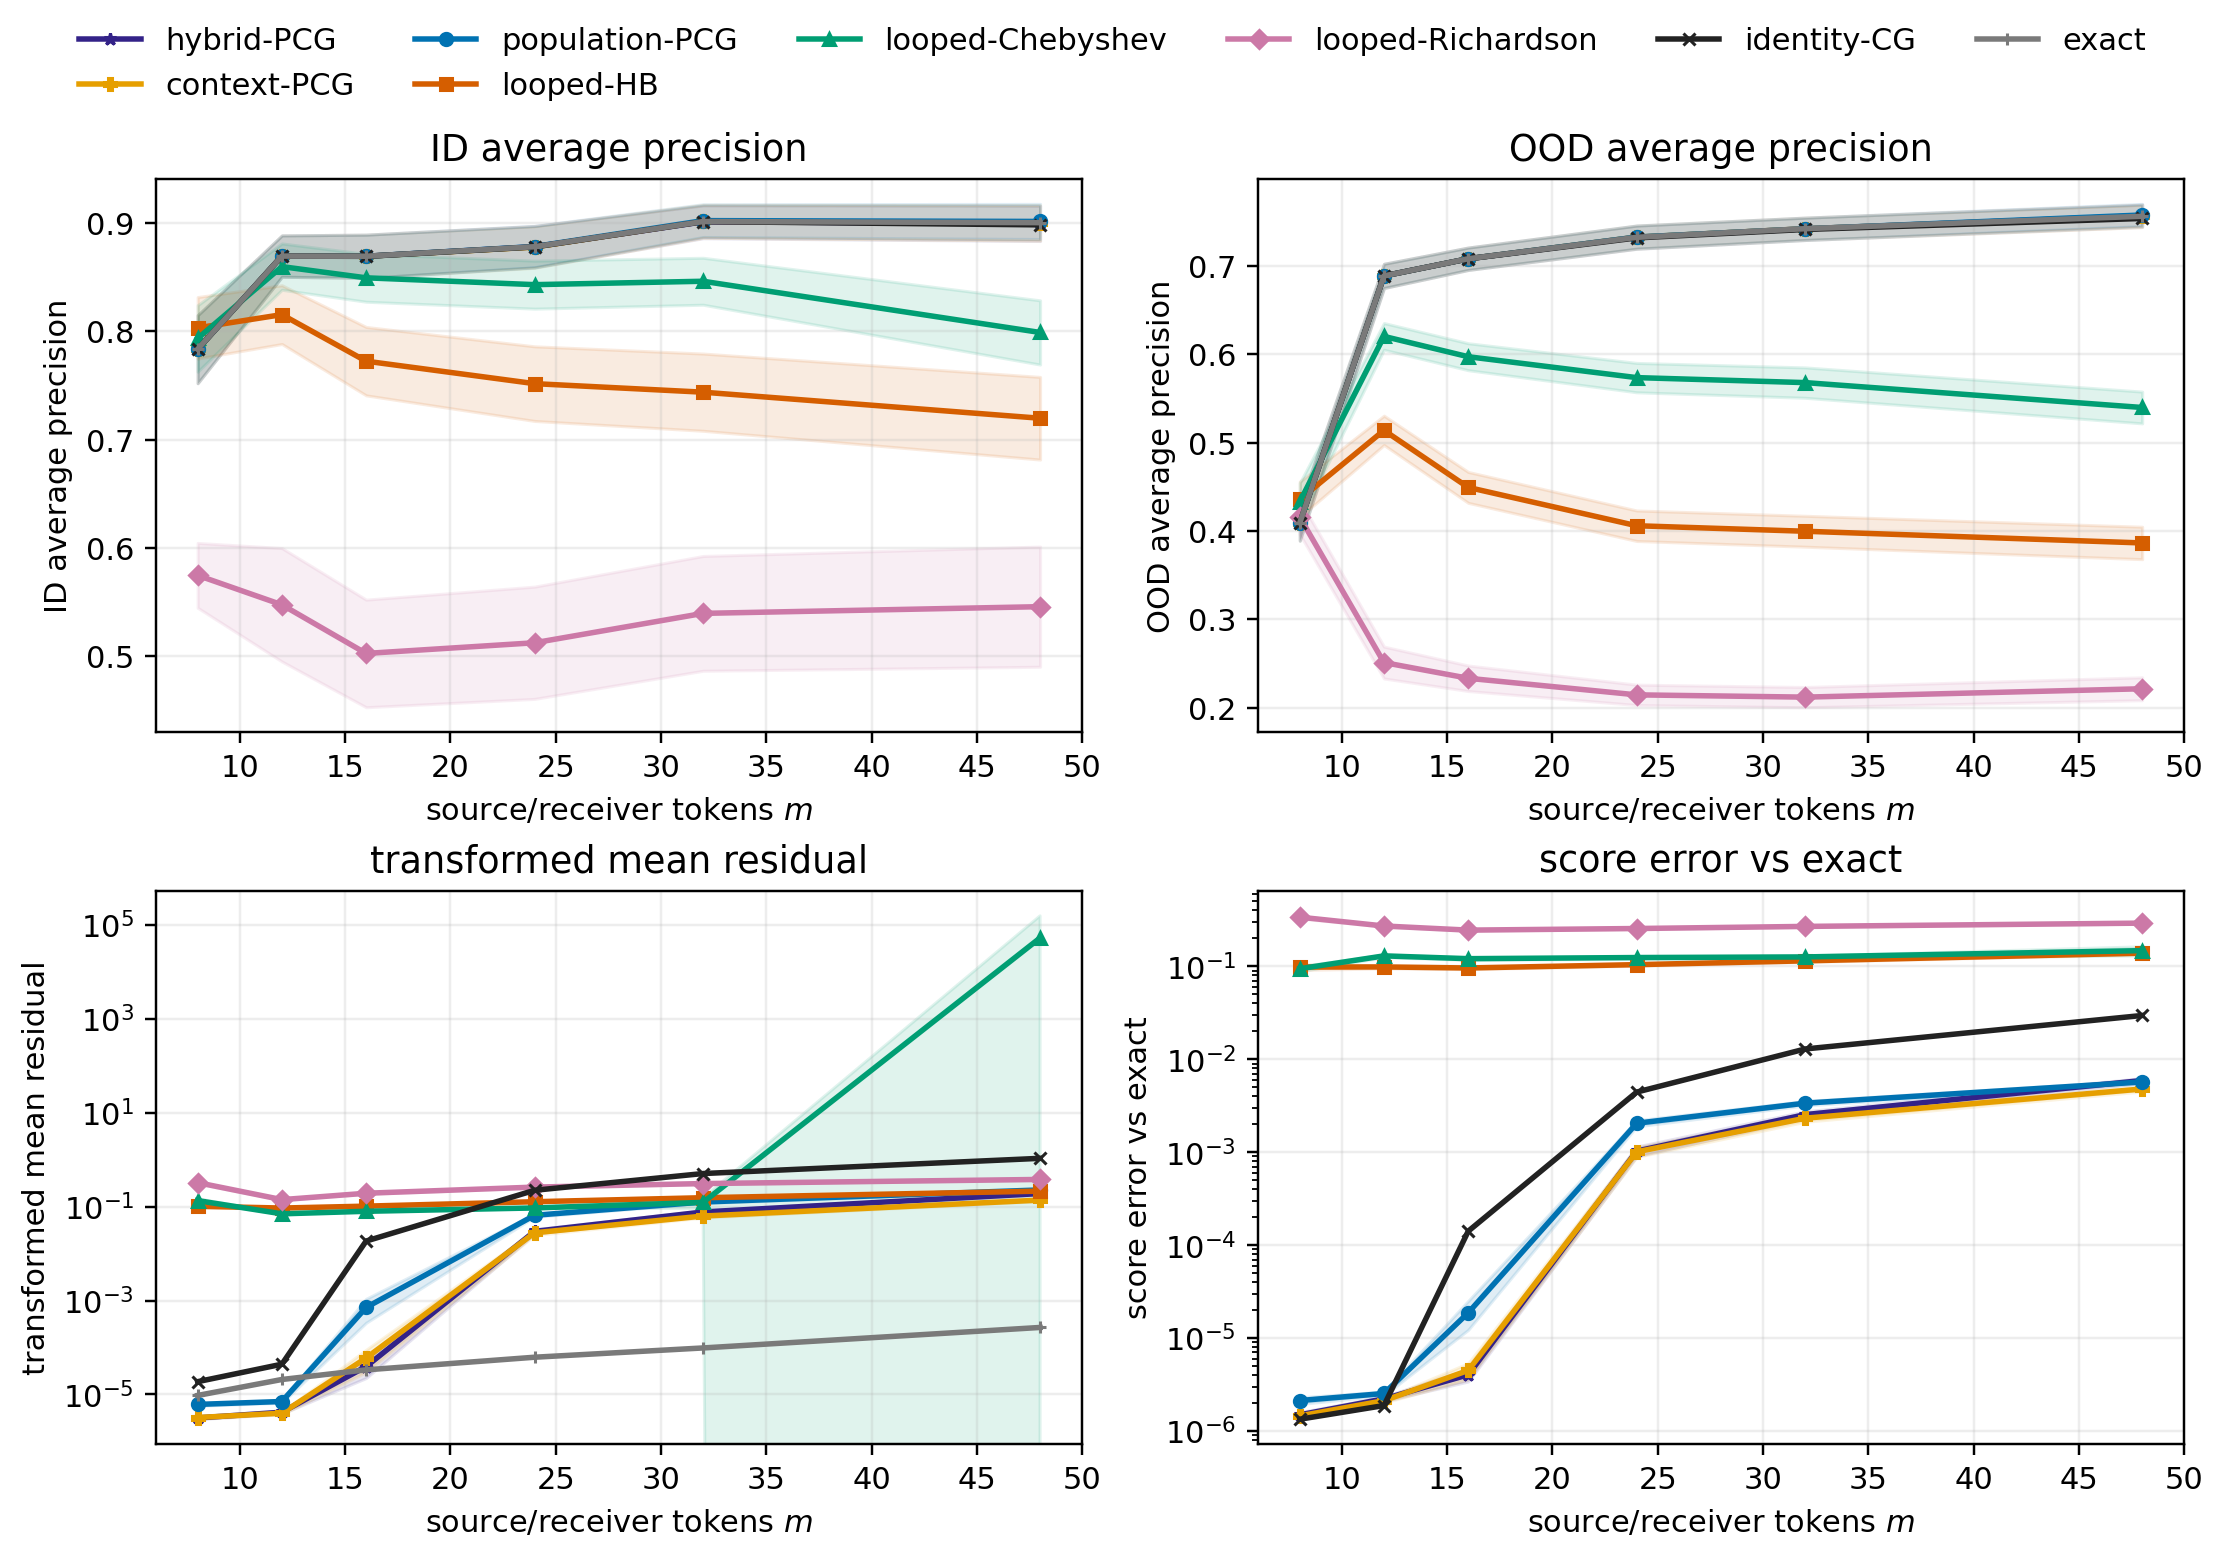
\includegraphics[width=0.88\textwidth,height=0.70\textheight,keepaspectratio]{scaling_context.png}
\par\vspace{-0.2em}
\small\color{orange}\textbf{Separation of effects.}\color{navy}\enspace
CG and PCG reach nearly the same localization AP; context-PCG mainly reduces numerical score error.
\end{frame}

\begin{frame}{A bigger foundation model is not the answer}
\begin{columns}[T,onlytextwidth]
\begin{column}{0.69\textwidth}
  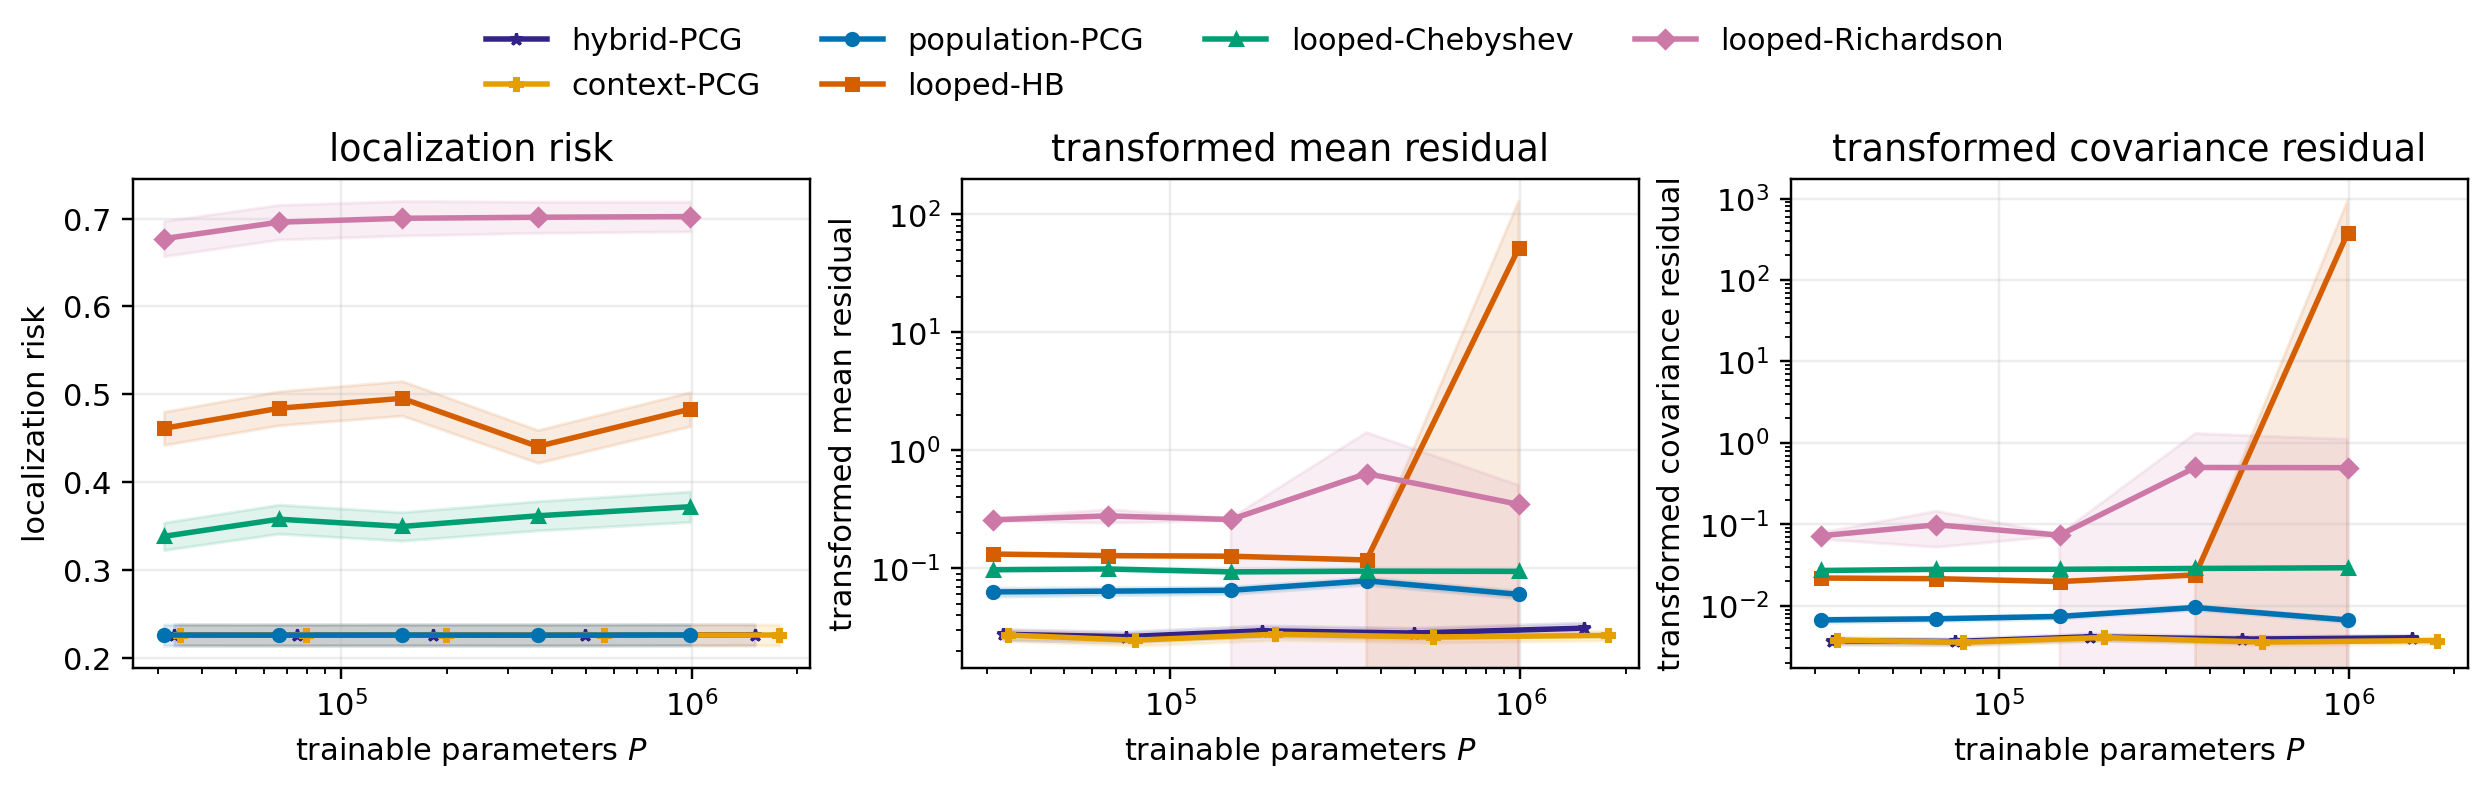
\includegraphics[width=\linewidth,height=0.79\textheight,keepaspectratio]{scaling_network.png}
\end{column}
\begin{column}{0.28\textwidth}
  \metric{Best context width}{64}
  \vspace{0.55em}
  \metric{Largest width}{512}
  \vspace{0.55em}
  \metric{Parameter ratio}{$22.45\times$}
  \vspace{0.8em}
  \begin{alertblock}{Observed plateau}
  Width 512 is 3.5\% worse than width 64. Capacity is not the bottleneck; the fixed modal basis is.
  \end{alertblock}
\end{column}
\end{columns}
\end{frame}

\begin{frame}{Bayesian UQ: numerical fidelity, not universal calibration}
\begin{columns}[T,onlytextwidth]
\begin{column}{0.57\textwidth}
  \centering
  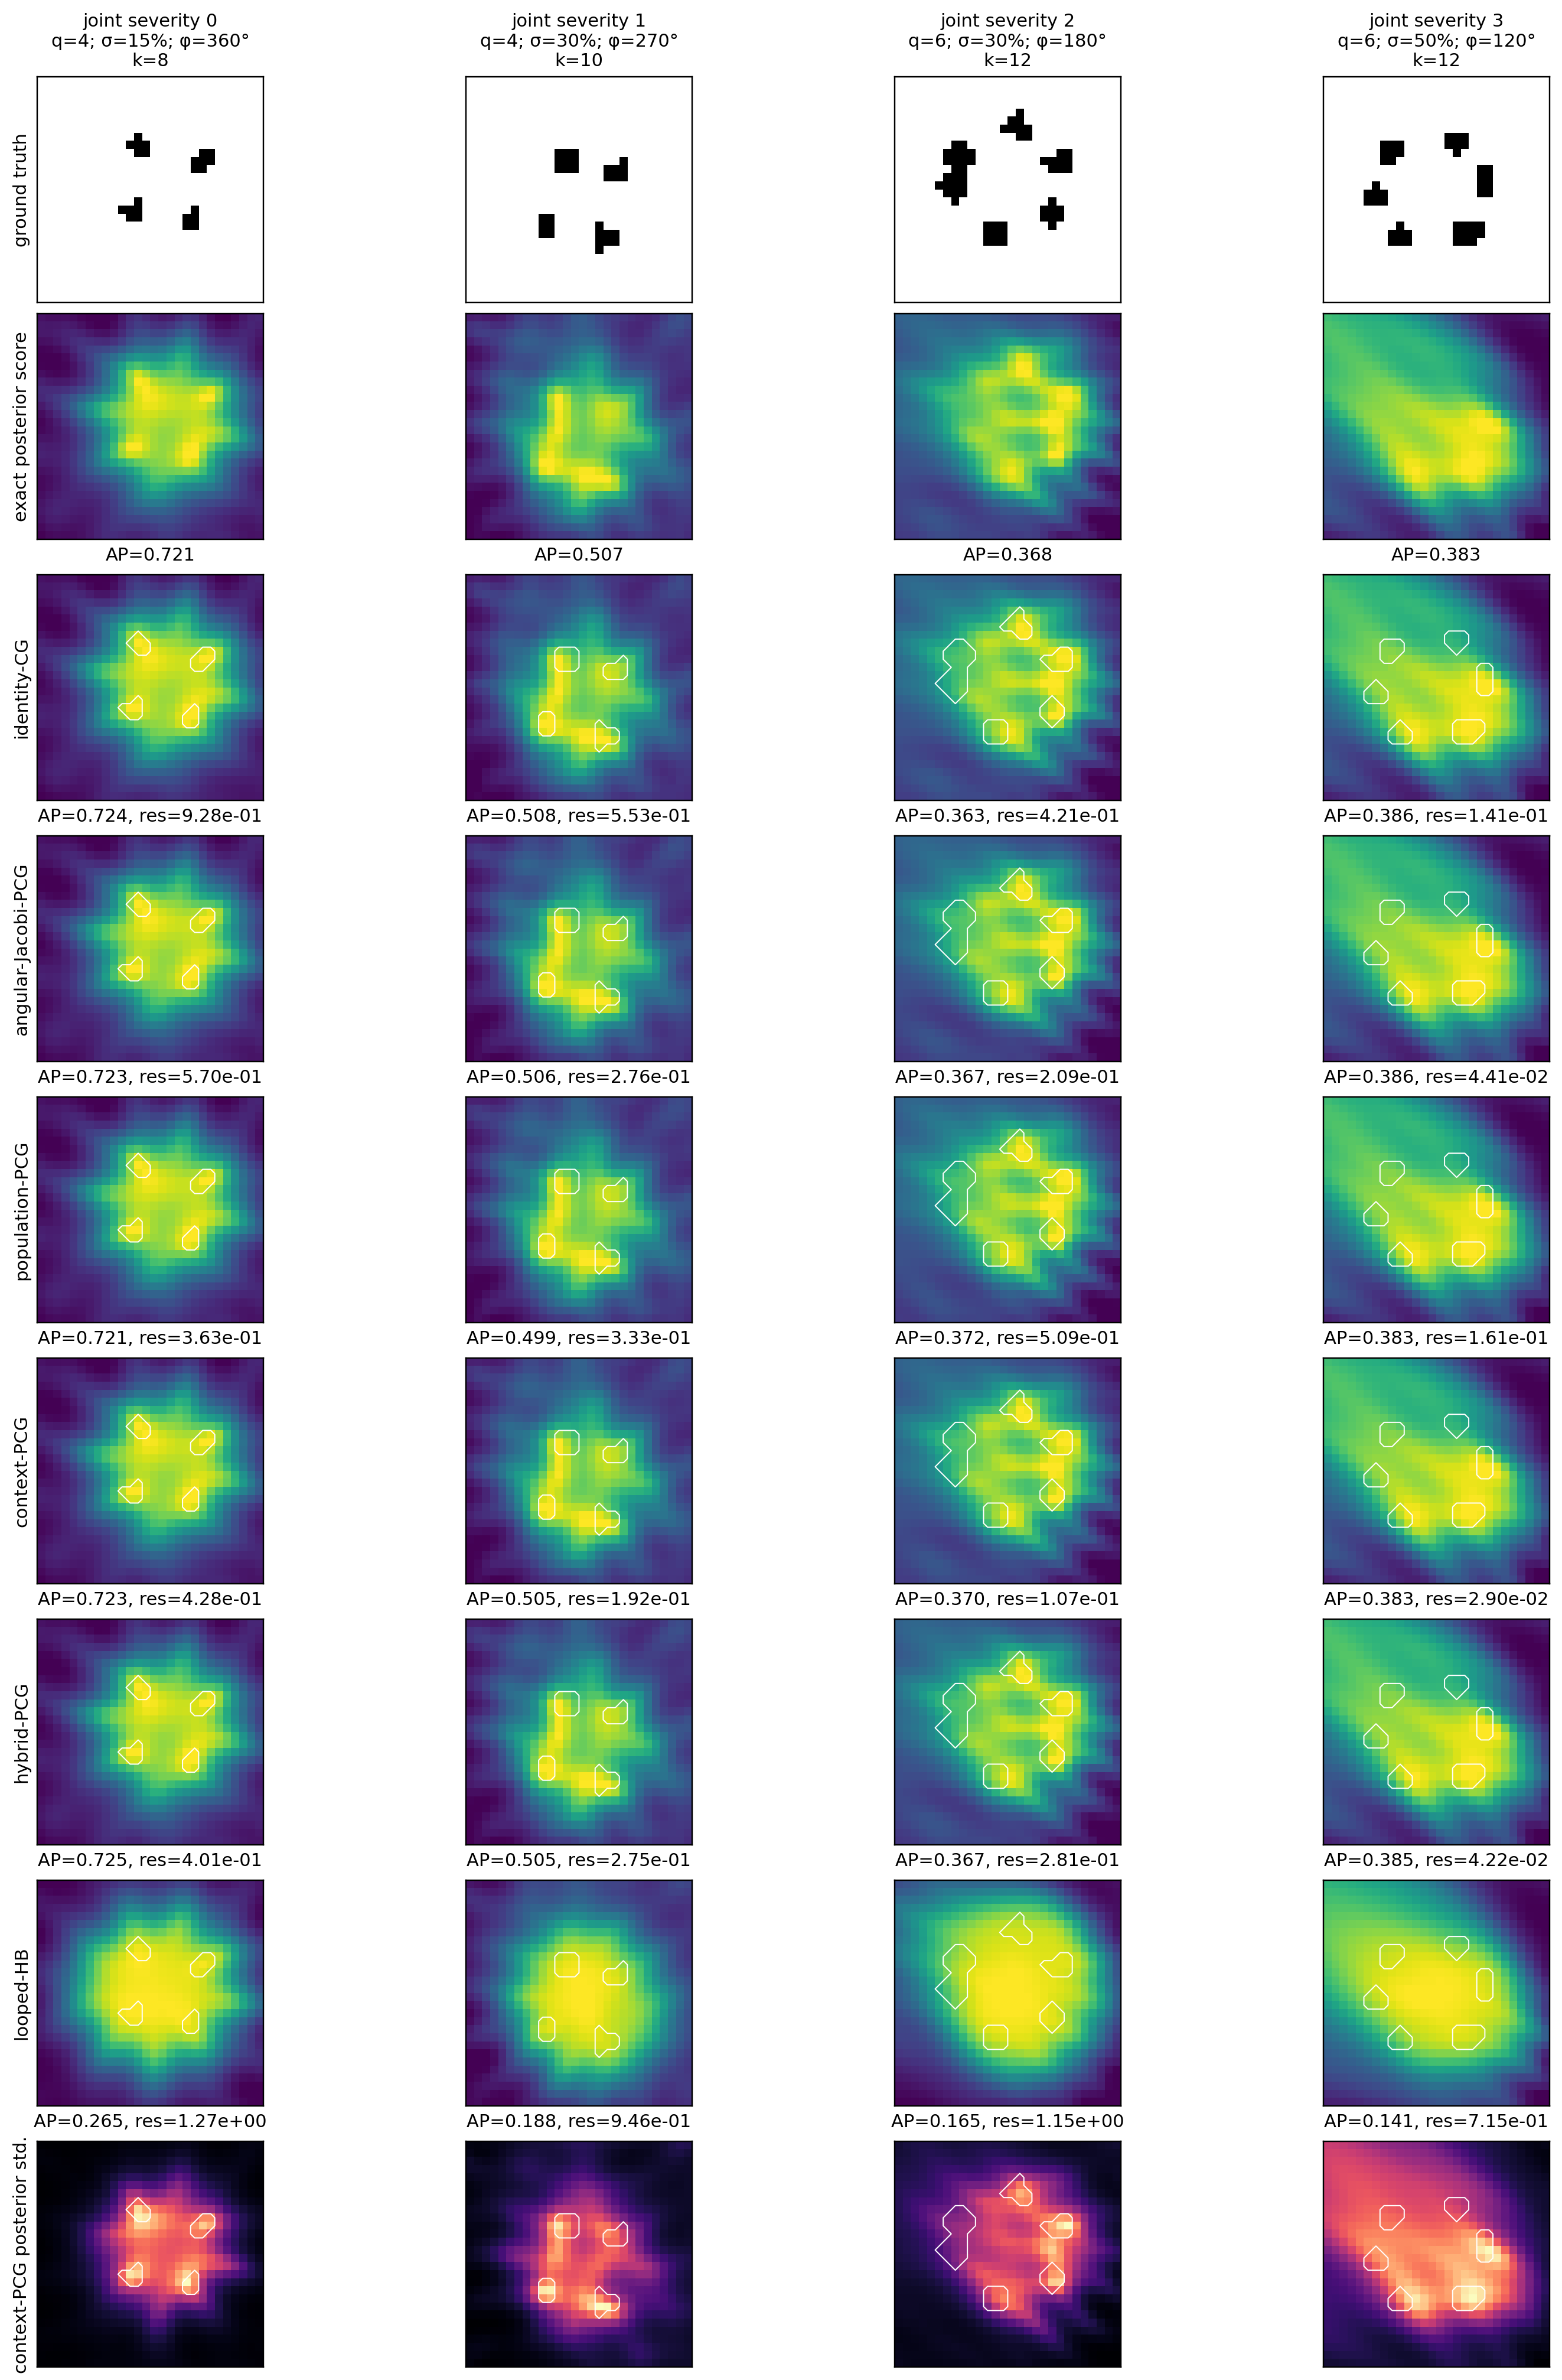
\includegraphics[width=\linewidth,height=0.68\textheight,keepaspectratio]{scaling_joint_reconstructions.png}
\end{column}
\begin{column}{0.40\textwidth}
  \small
  \begin{block}{What improves}
  \begin{itemize}\setlength\itemsep{0.1em}
    \item Mean and covariance solves approach the exact decoder.
    \item Numerical 95\% band coverage: $0.243\rightarrow0.873$ centrally.
  \end{itemize}
  \end{block}
  \begin{alertblock}{What does not}
  \begin{itemize}\setlength\itemsep{0.1em}
    \item Independent-geometry AP improves by only 0.0021.
    \item Extreme-shift UQ coverage gain collapses to zero.
  \end{itemize}
  This is numerical posterior fidelity, not frequentist obstacle coverage.
  \end{alertblock}
\end{column}
\end{columns}
\end{frame}

\begin{frame}{Generalization evidence and its scope}
\begin{columns}[T,onlytextwidth]
\begin{column}{0.69\textwidth}
  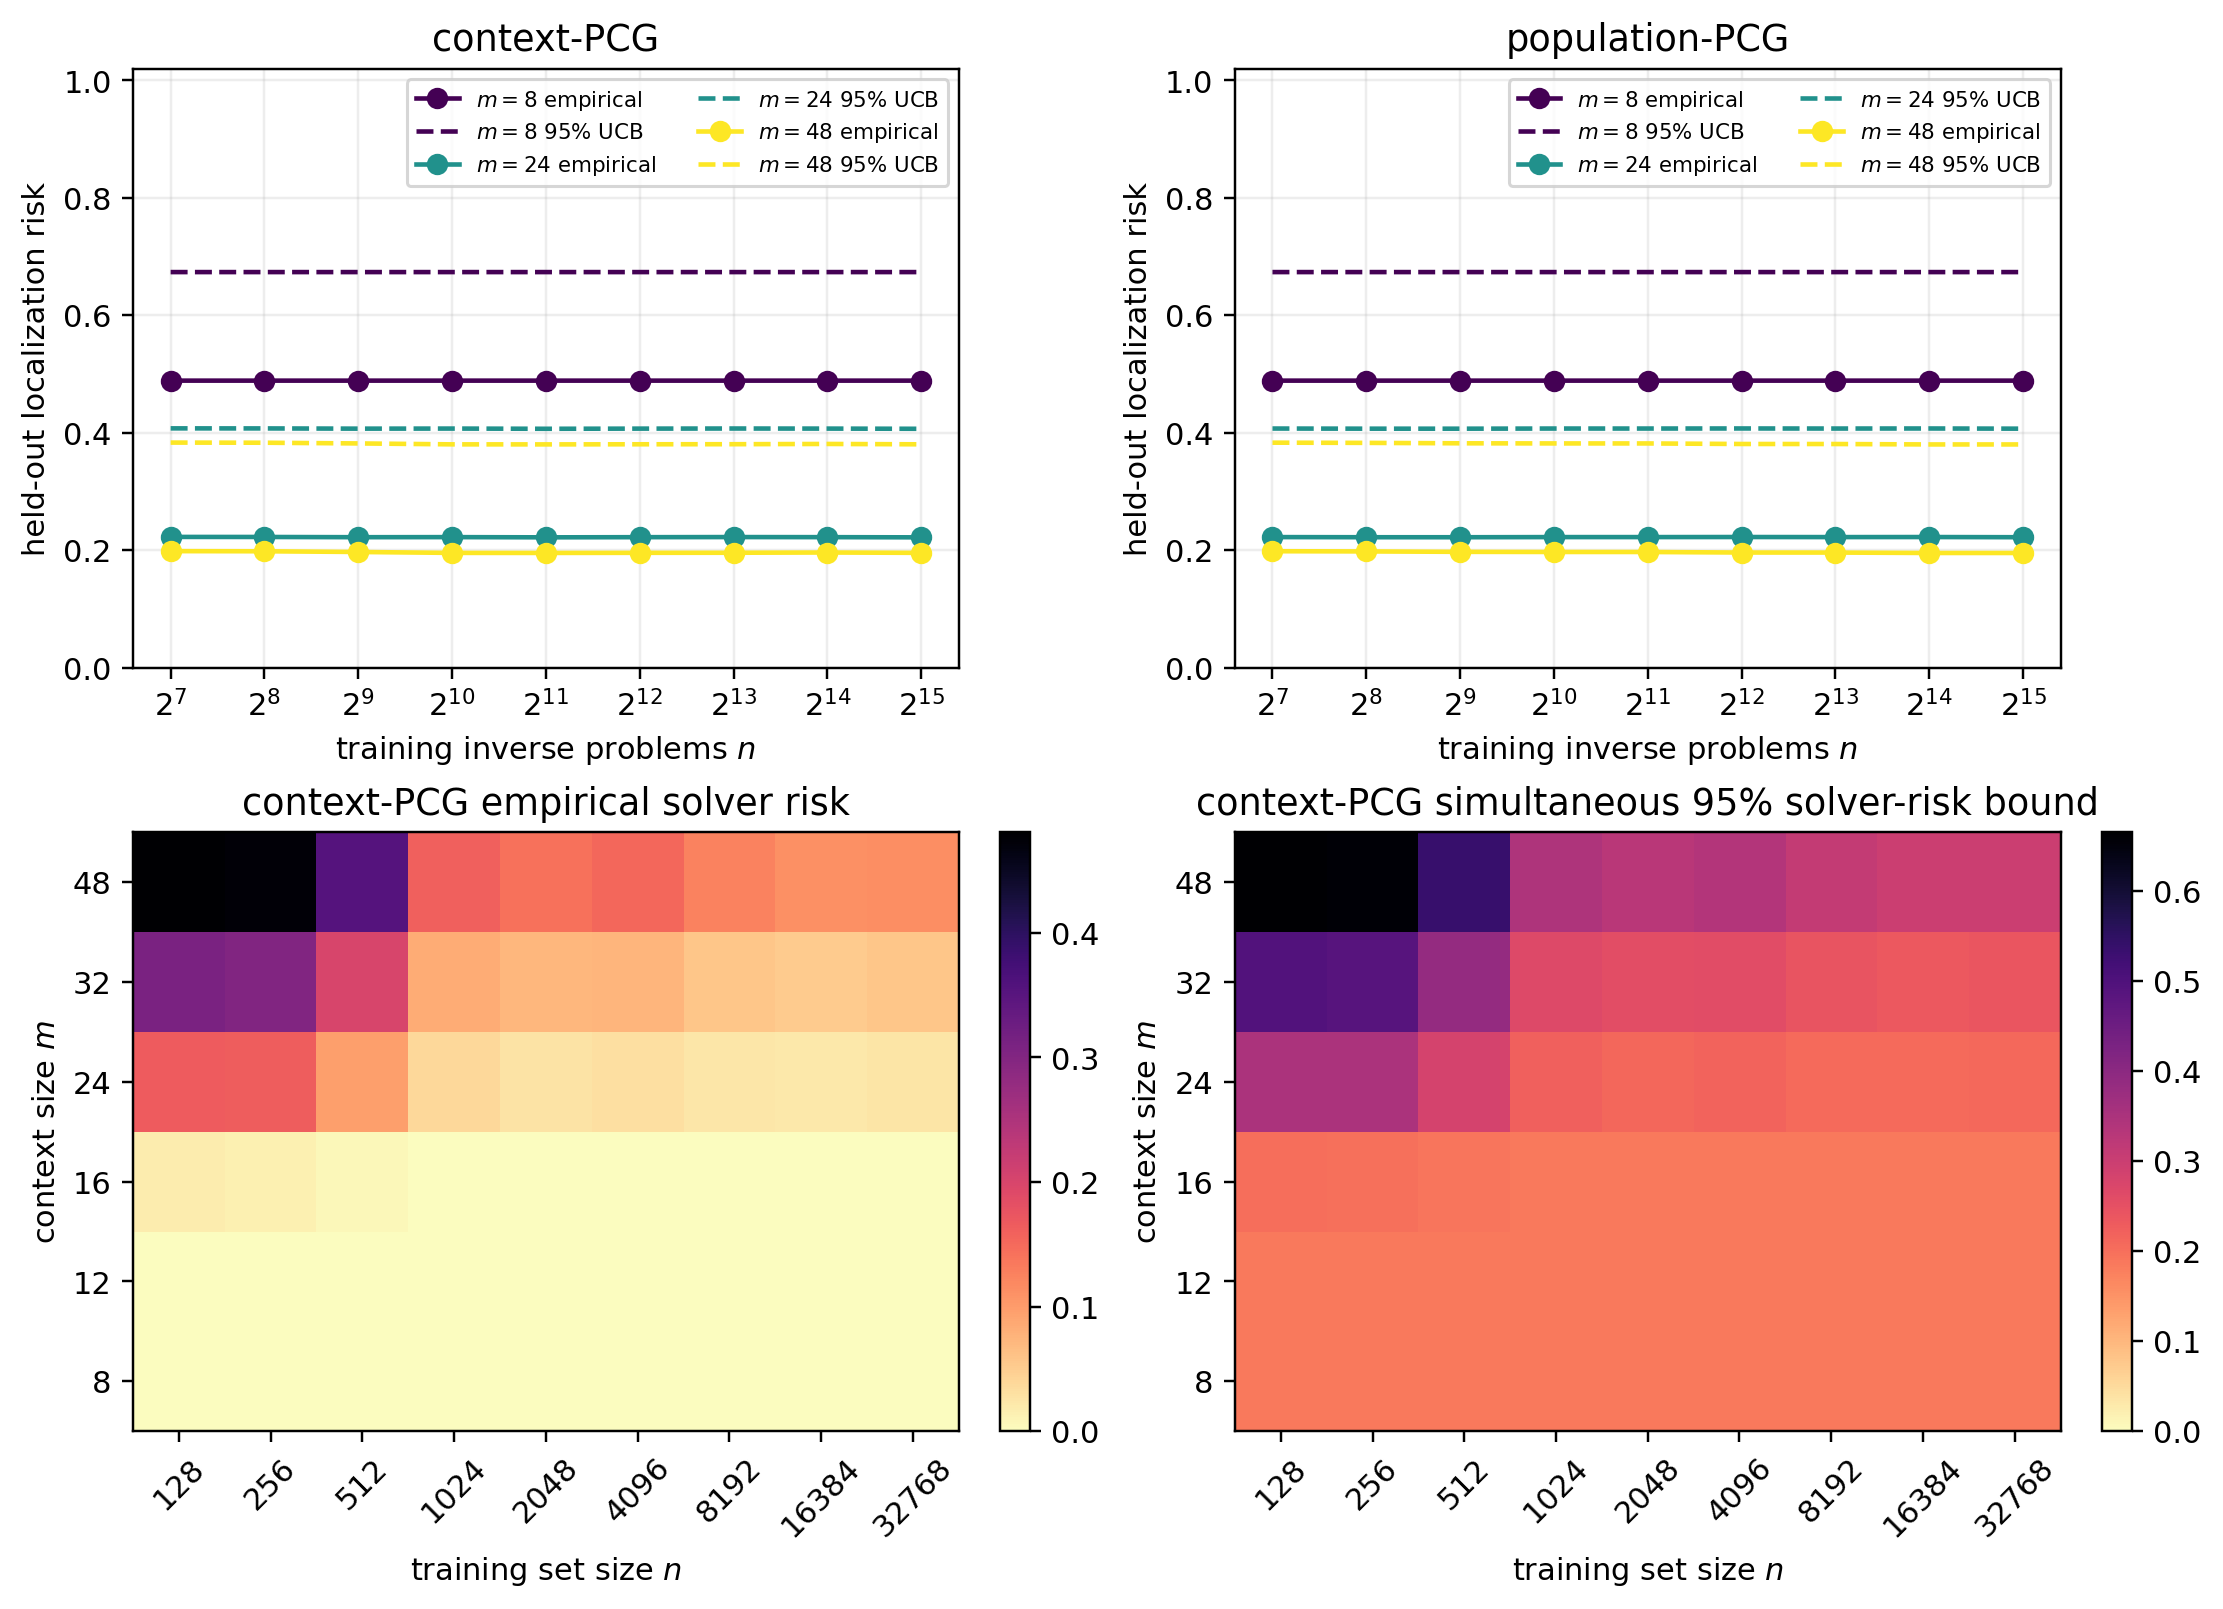
\includegraphics[width=\linewidth,height=0.65\textheight,keepaspectratio]{scaling_generalization_bounds.png}
\end{column}
\begin{column}{0.28\textwidth}
  \scriptsize
  \begin{block}{Certified quantity}
  Simultaneous 95\% held-out Hoeffding bounds over pre-specified settings.
  \end{block}
  \begin{block}{Correct sample size}
  Held-out task count sets the slack; training size only indexes the learned hypothesis.
  \end{block}
  \begin{alertblock}{Scope}
  Only for the sampled simulator distribution—not arbitrary geometries, experiments, or random-source LSM.
  \end{alertblock}
\end{column}
\end{columns}
\end{frame}

\begin{frame}{Conclusions: what context-PCG learned}
\small
\begin{columns}[T,onlytextwidth]
\begin{column}{0.57\textwidth}
  \begin{enumerate}\setlength\itemsep{0.25em}
    \item \textbf{Prompt-specific spectral weighting}: the current Hessian contains conditioning signal beyond shared acquisition geometry.
    \item \textbf{Finite-horizon adaptation}: learned gains improve clustering/RHS alignment beyond what scalar condition number predicts.
    \item \textbf{Robustness to unknown conditioning}: the gain over CG persists across every audited physical stress level.
    \item \textbf{Numerical Bayesian fidelity}: both mean and covariance solves improve, while physical localization remains acquisition-limited.
  \end{enumerate}
\end{column}
\begin{column}{0.39\textwidth}
  \begin{alertblock}{Current limitation}
  A diagonal controller in a fixed GP basis cannot rotate task-dependent eigendirections.
  \end{alertblock}
  \begin{block}{Next architecture}
  Learn block-Lanczos or polynomial rotations from RHS-weighted Ritz moments; preserve exact outer Krylov coefficients.
  \end{block}
  \begin{block}{One-line verdict}
  \textbf{Clearly better than ordinary CG; not yet universally better than informed analytic PCG.}
  \end{block}
\end{column}
\end{columns}
\end{frame}

\end{document}
